\documentclass[a4paper,12pt]{article}

% Packages
\usepackage[utf8]{inputenc}
\usepackage[T1]{fontenc}
\usepackage{amsmath}
\usepackage{subcaption}
\usepackage{graphicx}
\usepackage{hyperref}
\usepackage{media9}
\usepackage{tabularx}
\usepackage{mathtools}
\usepackage{pgfplots}
\pgfplotsset{compat=1.18}
\usepackage{xcolor}
\usepackage{geometry}
\usepackage[percent]{overpic} % in preamble
% \usepgfplotslibrary{external}
% \tikzexternalize[prefix=figures/]



\usepackage[authoryear]{natbib}

\definecolor{red}{rgb}{1,0,0}
\definecolor{blue}{rgb}{0,0,1}
\definecolor{green}{rgb}{0,0.5,0}
% Définir les marges
\geometry{
  a4paper,
  left=1.5cm,
  right=1.5cm,
  top=2cm,
  bottom=2cm
}

\title{Semi-active flapping foil harvests energy using evolutionary strategies}
\author{Brice Martin}
\date{\today}

\begin{document}

\maketitle

\section{Problem statement}\label{sec:pb_statement}
\begin{figure}[h]
  \centering
  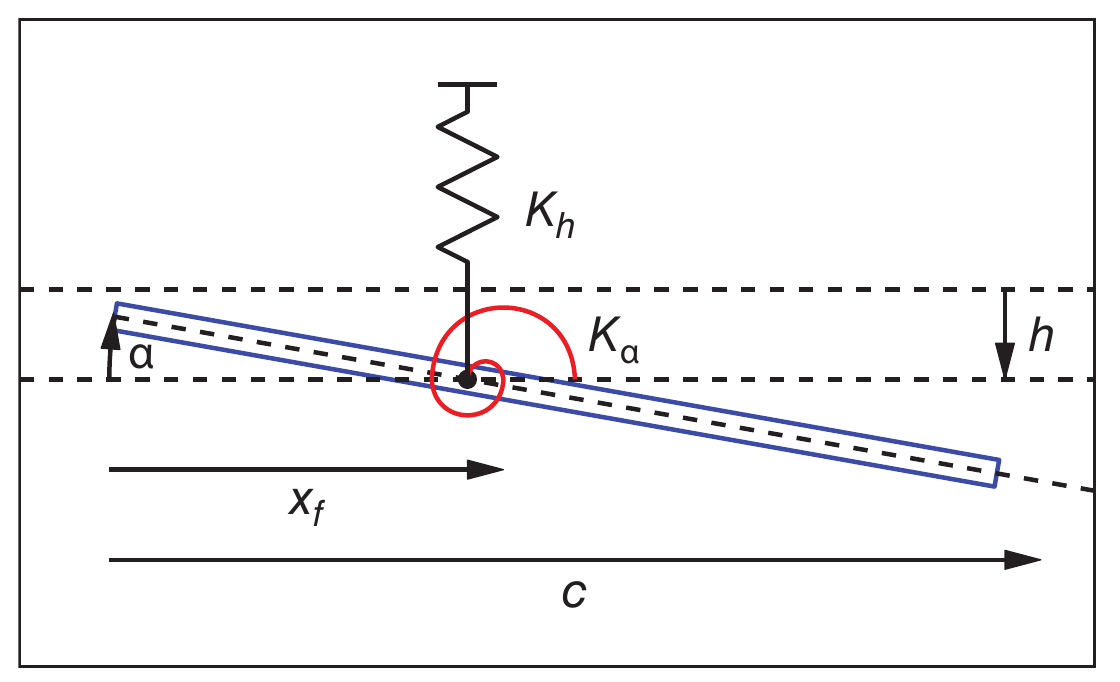
\includegraphics[width=0.5\textwidth]{images/2DoF_wing.png}
  \caption{Scheme of the problem.}
  \label{fig:scheme_pb}
\end{figure}

We consider a two-dimensional aerodynamic profile, modeled as an airfoil of chord \( c \), mass \( m \), and curvature profile \( \eta_{\mathcal{P}} \), flying at speed \( U \) in a fluid of density \( \rho \). 
The profile is allowed to pitch about its pitch axis, located at a distance \( x_f \) from the leading edge. 
The pitch angle is defined as the angle between the airfoil's chord and the horizontal axis. 
The plunge motion is defined as the vertical displacement of the pitch axis; a positive \( h \) represents a downward displacement. 
The airfoil is suspended from point \( x_f \) by an extension spring of stiffness \( K_h \). 
The system has one degree of freedom in the plunge motion and is modeled as a mass-spring-damper system:
\begin{equation}
  m \ddot{h} + c_h \dot{h} + K_h h = -l, 
\label{eq:plunge}
\end{equation}
where \( l \) is the aerodynamic load acting on the airfoil in the vertical direction, and \( c_h \) is the damping coefficient.  
The pitch motion is imposed in an open-loop fashion as:
\begin{equation}
  \alpha(t) = \alpha_0 + \alpha_1 \sin(\omega t) + \alpha_2 \sin(\omega_2 t) + \alpha_3 \sin(\omega_3 t),
\label{eq:alpha}
\end{equation}
where \( \alpha_0 \) is the mean pitch angle, and \( \alpha_1 \), \( \alpha_2 \), and \( \alpha_3 \) are the amplitudes of the first, second, and third harmonics, respectively.  
The corresponding frequencies are \( \omega \), \( \omega_2 \), and \( \omega_3 \), and their reduced frequencies are defined as
\[
k_i = \frac{\omega_i c}{2U}.
\]
A complete schematic of the system is depicted in Fig.~\ref{fig:scheme_pb}.

The objective of this study is to find the optimal kinematic parameters \( \{k_i, \alpha_j\}_{i \in [1,3],\, j \in [0,3]} \) and mass-spring-damper parameters \( m \), \( c_h \), and \( K_h \), such that the airfoil extracts the maximum power from the fluid flow.

An efficiency metric is defined based on three quantities: the power extracted from the flow, the power required to enforce the pitch motion, and the maximum extractable power.
The power extracted from the flow by the airfoil is given by
\[
P_e = l\, \dot{h},
\]
the cost of the imposed pitch motion is
\[
P_c = M_{x_f}\, \dot{\alpha}, \quad \text{with } P_c < 0,
\]
and the maximum extractable power is
\[
P_{\text{max}} = \frac{1}{4} \rho U^3 c^2.
\]
The efficiency metric is then defined as:
\begin{equation}
\eta = \int_0^T \frac{P_e + P_c}{P_{\text{max}}} \, dt,
\label{eq:efficiency}
\end{equation}
where \( T \) denotes one pseudo-period of the open-loop pitch motion.

The optimization problem can thus be formulated as finding the parameter vector
\begin{equation}
\theta = \left( \{k_i, \alpha_j\}_{i \in [1,3],\, j \in [0,3]},\, m,\, c_h,\, K_h \right)
\label{eq:theta}
\end{equation}
such that the efficiency \( \eta \) is maximized.

The aerodynamic loads \( l \) and \( M_{x_f} \) are computed using the LDVM  method, which is presented in the next section.


\section{Loads computation according to LDVM}

\subsection{Aerodynamic model}
The LESP-modulated Discrete Vortex Method (LDVM) is a numerical approach used to compute aerodynamic loads, introduced by \cite{ramesh2014discrete}.  
It is a medium-fidelity tool, valid under the assumptions of unsteady, incompressible, and inviscid (potential) flow, which in particular implies an infinite Reynolds number.  
These assumptions make the LDVM similar to the unsteady vortex lattice method (UVLM) \cite{katz_plotkin}. However, whereas the latter assumes that the flow remains attached to the airfoil's leading edge (i.e., it relies on a small-angle approximation), the LDVM is capable of modeling leading-edge flow separation that occurs at high angles of attack.

The method approximates the overall flow as the superposition of the incident flow \( \mathbf{U} \) and the induced velocities generated by a discrete set of vortex singularities.  
Among these vortices, \( N \) are located along the airfoil chord (bound vortices), \( N_{{TEV}} \) are shed from the trailing edge (TE), and \( N_{{LEV}} \) are shed from the leading edge (LE).  
In the following, we refer to the sets of bound, trailing-edge, and leading-edge vortices as \( \mathcal{P} \), \( \mathcal{TEV} \), and \( \mathcal{LEV} \), respectively.
We denote by \( \Gamma_{b,i} \) and \( \mathbf{x}_{b,i} \) the circulation and position of the \( i \)-th bound vortex,  
by \( \Gamma_{{TEV},j} \) and \( \mathbf{x}_{{TEV},j} \) the circulation and position of the \( j \)-th trailing-edge vortex,  
and by \( \Gamma_{{LEV},j} \) and \( \mathbf{x}_{{LEV},j} \) the circulation and position of the \( j \)-th leading-edge vortex.

% The velocity induced by the k-th vortex of circulation $\Gamma$ in a point $\mathbf{X}=(X,Z)$, $V_k(\mathbf{X})= u~\mathbf{e}_x, v~\mathbf{e}_z $ is given by:
% \begin{align}
% u &= \frac{\Gamma}{2\pi} \frac{Z - Z_k}{\sqrt{(X - X_k)^2 + (Z - Z_k)^2 + v_{core}^4}} \notag\\
% w &= -\frac{\Gamma}{2\pi} \frac{X - X_k}{\sqrt{(X - X_k)^2 + (Z - Z_k)^2 + v_{core}^4}},
% \end{align}
% where $(X_k, Z_k)$ are the coordinates of the vortex core, and $v_{core}$ is the core size of the vortex set to $0.02 c$.


The normal force \( F_N \) acting on the airfoil is obtained by integrating the pressure coefficient, modeled using Bernoulli’s equation, over the chord \citep{ramesh2014discrete}:
\begin{equation}
    F_N = \rho \left[ \int_0^c \left( U \cos(\alpha) + \dot{h} \sin(\alpha) + \left( \frac{\partial \phi_{LEV}}{\partial x} \right) + \left( \frac{\partial \phi_{TEV}}{\partial x} \right) \right) \gamma(x, t) \, dx
    + \int_0^c \frac{\partial}{\partial t} \left( \int_0^x \gamma(x_0, t) \, dx_0 \right) dx \right],
    \label{eq:FN_integral}
\end{equation}
where $\gamma$ represents the chordwise vorticity distribution on the airfoil, $\phi_{LEV}$ and $\phi_{TEV}$ are the potential functions of the LEV and TEV vortex induced flows. The chordwise vorticity distribution $\gamma(x)$ on the aerofoil is represented as a Fourier series:
\begin{equation}
    \gamma(\theta, t) = 2U \left[ A_0(t) \frac{1 + \cos\theta}{\sin\theta} + \sum_{n=1}^{\infty} A_n(t) \sin(n\theta) \right],
    \label{eq:gamma_fourier}
\end{equation}
where $\theta$ is a transformation variable related to the chordwise coordinate $x$ by $x = \frac{c}{2} (1 - \cos\theta)$, and $A_0(t), A_1(t), \ldots, A_n(t)$ being the time-dependent Fourier coefficients.
These are given as a function of the downwash $W(x, t)$ on the airfoil:
\begin{align}
    A_0(t) &= -\frac{1}{\pi} \int_0^{\pi} \frac{W(x, t)}{U} \, d\theta, \label{eq:A0}\\
    A_n(t) &= \frac{2}{\pi} \int_0^{\pi} \frac{W(x, t)}{U} \cos(n\theta) \, d\theta, \label{eq:An}
\end{align}
with the downwash given as:
\begin{equation}
    W(x, t) = \frac{\partial \eta}{\partial x} \left( U \cos\alpha + \dot{h} \sin\alpha + \frac{\partial \phi_{LEV}}{\partial x} + \frac{\partial \phi_{TEV}}{\partial x} \right)
    - U \sin\alpha - \dot{\alpha} (x - x_f) + \dot{h} \cos\alpha - \frac{\partial \phi_{TEV}}{\partial z} - \frac{\partial \phi_{LEV}}{\partial z}.
    \label{eq:W}
\end{equation}
The evaluation of the Fourier coefficients allows the airfoil's normal force to be simplified as follows:
\begin{align}
    F_N &= \rho \pi c U \left[ \left( U \cos\alpha + \dot{h} \sin\alpha \right) \left( A_0(t) + \frac{1}{2}A_1(t) \right)
    + c \left( \frac{3}{4} \dot{A}_0(t) + \frac{1}{4} \dot{A}_1(t) + \frac{1}{8} \dot{A}_2(t) \right) \right]\notag \\
    &+ \rho \int_0^c \left( \frac{\partial \phi_{LEV}}{\partial x} + \frac{\partial \phi_{TEV}}{\partial x} \right) \gamma(x, t) \, dx.
    \label{eq:FN_fourier}
\end{align}


The derivatives of the potential function occurring in Eqs.~\ref{eq:W};~\ref{eq:FN_fourier} need to be further detailed to compute the aerodynamic loads.
The definition of flow potentials states that $\partial \phi_{LEV}/\partial x_i(\textbf{x})$ (resp.~$\partial \phi_{TEV}/\partial x_i(\textbf{x})$) is equal to the component $x_i$, in the airfoil's coordinate system,  of the LEV-induced (resp.~TEV-induced) velocity on point $\textbf{x}$.
Consequently they can be written as:
\begin{align}
  &\frac{\partial \phi_{LEV}}{\partial x}=\sum_{i\in \mathcal{LEV}} U_i(\mathbf{x})\cos(\alpha)- W_i(\mathbf{x})\sin(\alpha),
  \frac{\partial \phi_{LEV}}{\partial z}=\sum_{i\in \mathcal{LEV}} U_i(\mathbf{x})\sin(\alpha)+ W_i(\mathbf{x})\cos(\alpha),\notag\\
  &\frac{\partial \phi_{TEV}}{\partial x}=\sum_{j\in \mathcal{TEV}} U_j(\mathbf{x})\cos(\alpha)- W_j(\mathbf{x})\sin(\alpha),
  \frac{\partial \phi_{TEV}}{\partial z}=\sum_{j\in \mathcal{TEV}} U_j(\mathbf{x})\sin(\alpha)+ W_j(\mathbf{x})\cos(\alpha),
  \label{eq:velocity_wake_lev}
\end{align} 
where $U_k(\textbf{x}),W_k(\textbf{x})$ are respectively the x- and z- velocity induced by the k-th vortex of circulation $\Gamma_k$ and located in $\textbf{x}_k=(x_k,z_k)$. 
They are given as:
\begin{align}
U_k(x,z) &= \frac{\Gamma_k}{2\pi} \frac{z - z_k}{\sqrt{((x - x_k)^2 + (z - z_k)^2)² + v_{core}^4}} \notag\\
W_k(x,z) &= -\frac{\Gamma_k}{2\pi} \frac{x - x_k}{\sqrt{((x - x_k)^2 + (z - z_k)^2)^2 + v_{core}^4}},
\label{eq:velocity_formula}
\end{align}
where $v_{core}$ is the core size of the vortex set to $0.02 c$.

Equations~\ref{eq:velocity_wake_lev} and \ref{eq:velocity_formula} state that the $LEV$ and $TEV$-induced velocities are parameterized by (i) the number of $LEV$ and $TEV$ vortices, (ii) the vortex circulations,  and (iii) the vortex core positions.

In an LDVM method, $TEV$ vortex shedding occurs at each time step, whereas $LEV$ vortex shedding  occurs if and only if a critical value of the so-called leading-edge suction parameters (LESP) is exceeded.
The LESP is a  measure of the suction at the leading edge and it has been shown \citep{ramesh_unsteady_2013,ramesh2011augmentation} that LEV shedding always occurs at the same critical value of LESP (LESPc), regardless of motion kinematics.
\cite{ramesh2014discrete} explains that LESPc value depends only on the airfoil and the Reynolds number.
According to \cite{ramesh2014discrete}, the instantaneous LESP can be computed as $LESP(t)=A_0(t)$, and Consequently $LEV$ shedding  occurs if $|A_0|$ exceeds $|LESPc|$.

The strength of the TEV shed at the current time step is calculated to enforce Kelvin’s condition.
\begin{equation}
    \Gamma_b(t) + \sum_{m=1}^{N_{TEV}} \Gamma_{TEV,m} + \sum_{n=1}^{N_{LEV}} \Gamma_{LEV,n} = 0
    \label{eq:kelvin_circulation}
\end{equation}
where $\Gamma_b$ is the bound circulation calculated by integration of the distribution of $\gamma$ over the airfoil chord. It satisfies:
    $\Gamma_b = U c \pi \left[ A_0(t) + \frac{1}{2} A_1(t) \right]$.
If there is LEV shedding, the strength  of the $LEV$ shed at the current time step is determined such that  the instantaneous LESP value is equal to the LESPc: $A_0(t)=LESPc$, if $A_0(t)<LESPc$, then no LEV shedding is performed.
Note that two equations need to be satisfied in case of LEV shedding, whereas only one equation is needed if no LEV is shed.
Once computed, the LEV and TEV circulations remain constant because the fluid is considered inviscid.

The position of the vortex cores are computed by advecting the $TEV$ vortices and the $LEV$ vortices  by the 
total flow velocity: $\textbf{V}(\textbf{x})= \sum_{i\in \mathcal{P}} \textbf{V}_{i}(\textbf{x}) + \sum_{i\in \mathcal{TEV}} \textbf{V}_{i}(\textbf{x}) + \sum_{i\in \mathcal{LEV}} \textbf{V}_{i}(\textbf{x})$ using a first order difference scheme.
The position of the $TEV$ or $LEV$ vortex shed at the current time step is given by:
\begin{equation}
    (x, z)_{TEV_i/LEV_i} = (x, z)_{TE/LE} + \frac{1}{3} \left[ (x, z)_{TEV_{i-1}/LEV_{i-1}} - (x, z)_{TE/LE} \right]
\end{equation}
where $(x, z)_{TE/LE}$ denotes the coordinates of the TE or LE, and $(x, z)_{TEV_{i-1}/LEV_{i-1}}$ denotes the position of the previously shed TEV or LEV vortex. The position of the first shed vortex, i.e., first shed TEV or first shed LEV after LEV shedding stops, is determined using the velocity at the shedding edge.



The normal force coefficient $C_N$ is calculated by dividing $F_N$ by $(1/2)\rho U^2 c$. The lift and drag coefficients of the airfoil are derived from $C_N$ and the leading-edge suction force $F_S$ as:
\begin{align}
    C_L &= C_N \cos\alpha + C_S \sin\alpha, \label{eq:CL}\\
    C_D &= C_N \sin\alpha - C_S \cos\alpha. \label{eq:CD},
\end{align}
where $C_S=2F_S/\rho U^2c$ is derived from a leading-edge suction force, $F_S$, acting axially to the airfoil, it is given by the Blasius formula \citep{ramesh2014discrete}:
\begin{equation}
    F_S = \rho \pi c U^2 A_0^2.
    \label{eq:FS_blasius}
\end{equation}


The moment on the airfoil is given by:
\begin{align}
    m_{x_f} &=  x_{\text{ref}} F_N - \rho \pi c^2 U \left[ (U \cos\alpha + \dot{h} \sin\alpha) \left( \frac{1}{4}A_0(t) + \frac{1}{4}A_1(t) - \frac{1}{8}A_2(t) \right) \right. \notag \\
    &\quad \left. + c \left( \frac{7}{16} \dot{A}_0(t) + \frac{11}{64} \dot{A}_1(t) + \frac{1}{16} \dot{A}_2(t) - \frac{1}{64} \dot{A}_3(t) \right) \right] \notag \\
    &\quad - \rho \int_0^c \left( \frac{\partial \phi_{LEV}}{\partial x} + \frac{\partial \phi_{TEV}}{\partial x} \right) \gamma(x, t) x \, dx.
    \label{eq:moment}
\end{align}



\subsection{Model Validation}
\begin{figure}[h]
    \centering
    \begin{tikzpicture}
        \begin{axis}[
            width=0.5\textwidth,
            xlabel={Time},
            ylabel={$\alpha$},
            grid=major,
        ]
        \addplot table [x index=0, y index=1] {motion_pr_amp45_k0.2.dat};
        \end{axis}
    \end{tikzpicture}
    \caption{Pitch motion $\alpha$ as a function of time.}
    \label{fig:eldredge_function}
\end{figure}

\subsubsection{Validation of our implementation of the LDVM}

The LDVM method has already been extensively validated against high-fidelity simulations in \cite{ramesh2014discrete}.  \cite{ramesh2014discrete} propose an implementation of the LDVM in Fortran 95. 
In this work, the loads produced by the LDVM method are used to compute the heave motion (Eq.~\ref{eq:plunge}) and the optimization target, $\eta$. 
To facilitate communication between the LDVM method, the dynamical model, and the optimization algorithm, the LDVM has been reimplemented in Python. This section presents the results of the Python implementation compared to those of the LDVM method implemented in Fortran 95.





The LDVM method is used to calculate the aerodynamic loads on a SD7012 airfoil, with a chord $c=1$, at a Reynolds number of $30000$. For this particular airfoil at this Reynolds number, the $LESPc$ is $0.18$.
The airfoil is subjected to a pitch motion with a maximal amplitude of $45^\circ$ for a duration of seven seconds. The time step is set to $\Delta t = 0.014$ seconds.
The airfoil's pitch angle function is defined as the Eldredge function \cite{eldredge2009computational}:
\begin{equation}
\alpha(t) = \ln \left[
    \frac{\cosh\left( \frac{a U_\infty (t - t_1)}{c} \right)
    \cosh\left( \frac{a U_\infty (t - t_4)}{c} \right)}
    {\cosh\left( \frac{a U_\infty (t - t_2)}{c} \right)
    \cosh\left( \frac{a U_\infty (t - t_3)}{c} \right) }
\right],
\end{equation}
where $a=2$ is a free parameter that determines the smoothing at the corners, and the times $t_1$ to $t_4$ are defined as:
$t_1 = \text{time from reference 0 until start of ramp}, t_2 = t_1 + \frac{A}{2K}, t_3 = t_2 + \frac{\pi A}{4K} - \frac{A}{2K},
    t_4 = t_3 + \frac{A}{2K}$, where $A$ is the amplitude of pitch (in radians) or plunge, and $K$ is the non-dimensional pitch/plunge rate.
The pitch angle function is represented in Fig.~\ref{fig:eldredge_function}.
\begin{figure}
  \centering
  \begin{overpic}[width=0.98\textwidth]{images/ldvm_validation.pdf}
      \put(10,70){{(a)}} % Adjust (x,y) as needed
    \put(60,70){{(b)}}

      \put(10,34){{(c)}} % Adjust (x,y) as needed
    \put(60,34){{(d)}}
  \end{overpic}
  \caption{Validation of the LDVM implementation. (a) shows the profile (\textcolor{black}{-----}), its interpolation ($\color{blue}{\cdot \cdot}$) and the camber line (\textcolor{green}{-----}). (b), (c), (d) show respectively $C_L$, $C_D$, $C_m$ obtained with the fortran implementation (\textcolor{blue}{-~-~-}) and our python implementation (\textcolor{red}{-----}).}
  \label{fig:validation_ldvm}
\end{figure}

The LDVM method is used to compute the aerodynamic loads on the SD7012 airfoil, and the results are compared to  that obtained with the Fortran implementation of the LDVM method. These results are presented in Fig.~\ref{fig:validation_ldvm}.
The lift, drag, and moment coefficients obtained with the Python implementation (red lines) are shown to be in good agreement with those obtained with the Fortran implementation (blue lines).
However, the signals produced by the two implementations are noisy for $5\leq t\leq6$, and the two implementations produce slightly different signals during this time span.

The video \textit{ldvm\_validation.mp4} shows the temporal evolution of the positions and circulations of the bound, TEV, and LEV vortices during pitch motion. It compares the results produced by the Python and Fortran implementations of the LDVM method. Similar flow topologies are produced by the two implementations.
For $t^*=5.0$, it can be seen that one high intensity vortex belonging to the LEV has a different trajectory in the two implementations.
This may explain the slightly different signals observed in Fig.~\ref{fig:validation_ldvm} for $5\leq t\leq6$.









\subsection{Validation of the dynamical model}

A second validation of the implementation is performed on a two-dimensional aeroelastic system with two degrees of freedom: pitch and plunge.
This system is modeled using a set of ordinary differential equations derived from Lagrange's equations.
\begin{equation}
  \underbrace{\left(\begin{array}{ccc}
    m & S \\
    S & I_\alpha \\
    \end{array} \right)}_{\boldsymbol{A}}\left(\begin{array}{c}
    \ddot{h} \\
    \ddot{\alpha} \\
    \end{array}\right)+\underbrace{\left(\begin{array}{ccc}
      c_h & 0  \\
      0 & c_\alpha \\
      \end{array}\right)}_{\boldsymbol{C}}\left(\begin{array}{l}
      \dot{h} \\
      \dot{\alpha} \\
      \end{array}\right)\underbrace{\left(\begin{array}{ccc}
    K_h & 0 \\
    0 & K_\alpha \\
    \end{array}\right)}_{\boldsymbol{E}}\left(\begin{array}{l}
    h \\
    \alpha \\
    \end{array}\right)=\left(\begin{array}{c}
    -l \\
    m_{x f} \\
    \end{array}\right).
\label{eq:system}
\end{equation}
The parameters of the system are set as follows:
\begin{align*}
\rho       &= 1.225 \quad \text{kg/m}^3 && \text{(air density)} \\
c          &= 0.15 \quad \text{m}       && \text{(chord length)} \\
b          &= \frac{c}{2} = 0.075 \quad \text{m} && \text{(semi-chord)} \\
\text{span} &= 0.45 \quad \text{m}      && \text{(span)} \\
x_f        &= 0.25\,c = 0.0375 \quad \text{m} && \text{(elastic axis location)} \\
m          &= 3.0 \quad \text{kg}       && \text{(mass)} \\
I          &= \frac{m}{3}\left(c^2 - 3c x_f + 3x_f^2\right) && \text{(moment of inertia)} \\
S          &= m\left(\frac{c}{2} - x_f\right) && \text{(static moment about elastic axis)} \\
K_h        &= 200 \quad \text{N/m}      && \text{(heave stiffness)} \\
K_\alpha   &= 4 \quad \text{N/rad}      && \text{(pitch stiffness)} \\
D_h        &= \frac{K_h}{1000} = 0.2 \quad \text{N/(m$\cdot$s)} && \text{(heave damping)} \\
D_\alpha   &= \frac{K_\alpha}{1000} = 0.004 \quad \text{N/(rad$\cdot$s)} && \text{(pitch damping)} \\
a          &= \frac{x_{CG}}{b} && \text{(distance between mid-chord and CE, nondimensional).}
\end{align*}
The system \ref{eq:system} is integrated using the RK45 method implemented in the \texttt{scipy} library.

\cite{dimitriadis2017introduction} provides a model for this aeroelastic system, in which the system dynamics are written as in Eq.~\ref{eq:system} and the loads are computed according to Theodorsen's equations \citep{theodorsen1935general}.
The lift is given by:
\begin{equation}
    l=\rho b^2(U\pi\dot{\alpha}+\pi\ddot{h}-\pi ba\ddot{\alpha}- U T_4 \dot{\beta}-T_1b\ddot{\beta}) +2 \pi \rho b U C(k) w, 
    \label{Eq:lift}
\end{equation}
and the moment follows:
\begin{align}
    m_{x_f}&=-\rho b^2 \left(-a\pi b \ddot{h} +\pi b^2\left(\frac{1}{8}+a^2 \right)\ddot{\alpha} -(T_7+(c_h-a)T_1)b^2\ddot{\beta}\right)\notag\\
    &-\rho b^2 \left( \pi \left(\frac{1}{2}-a\right) U b\dot{\alpha} +\left( T_1-T_8-(c_h-a)T_4+\frac{T_{11}}{2}\right) Ub \dot{\beta}\right)\notag\\
    & - \rho b^2 (T_4+T_{10}) U^2 {\beta} + 2 \rho U b^2 \pi \left(a +\frac{1}{2}\right) C(k) \omega,
    \label{Eq:moment}
\end{align}
where $T_1, T_4, T_7, T_8, T_{10}, T_{11}$ are Theodorsen's parameters and $C$ is the Theodorsen's function \citep{theodorsen1935general}.
Theodorsen's model makes similar assumptions to the LDVM method; it is also valid for unsteady incompressible potential flow.
However, it differs in that it does not model flow separation at the leading edge and assumes sinusoidal pitch and plunge motion.
To account for this difference, an arbitrary high $LESPc$ is set to $50.0$ so that LEV shedding does not occur in the LDVM method. Consequently, the two models have the same assumptions and can be compared.
However, note that the LDVM model is of higher fidelity because it does not make restrictive assumptions about the pitch and plunge motions, unlike Theodorsen's model.

We validate our implementation of the LDVM and the dynamical equation (Eq.~\ref{eq:plunge}) by comparing the pitch and plunge motions resulting from the integration of Eq.~\ref{eq:system} and the loads obtained using either the LDVM method or Theodorsen's model.
In order to compare the two methods, we consider several flow speed values $U =5,12,15.3 m/s$ and compare the pitch and plunge motions obtained usinf the LDVM method and the Theodorsen's model, when $\alpha$ is initialized to $0$ and $h$ to $0.1c$.
The results are presented in Fig.~\ref{fig:validation_dynamical_model}.

The results show that the plunge motion $h$ obtained with the LDVM method (red line) and the Theodorsen's model (blue line) are in good agreement for $U = 5.0,12.0$.
However, for $U=15.3 m/s$, the pitch and plunge motions obtained with the LDVM method  differ greatly from those obtained with the Theodorsen's model. This is because flutter instability is triggered for $U\approx=15.3$, so slight discrepancies in the loads can result in significantly different motions.

\begin{figure}
  \centering
  \begin{subfigure}[]{0.48\textwidth}
    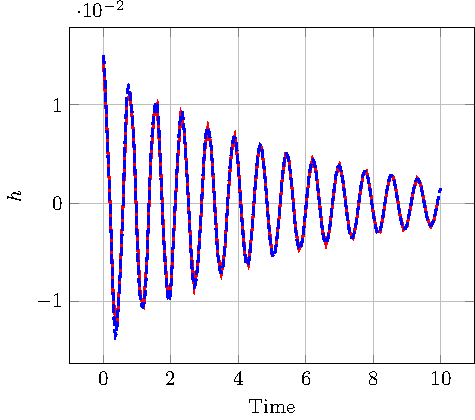
\includegraphics[width=\textwidth]{figures/fig_h_comparison_U_5.pdf}
    \caption{Plunge motion $h$ for $U=5 m/s$.}
  \end{subfigure}
  \begin{subfigure}[]{0.48\textwidth}
    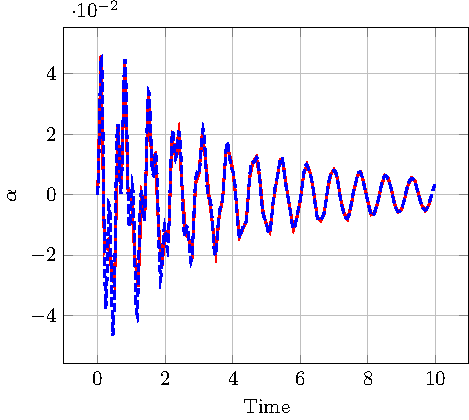
\includegraphics[width=\textwidth]{figures/fig_alpha_comparison_U_5.pdf}
  \caption{Pitch motion $\alpha$ for $U=5 m/s$.}
  \end{subfigure}
  \begin{subfigure}[]{0.48\textwidth}
    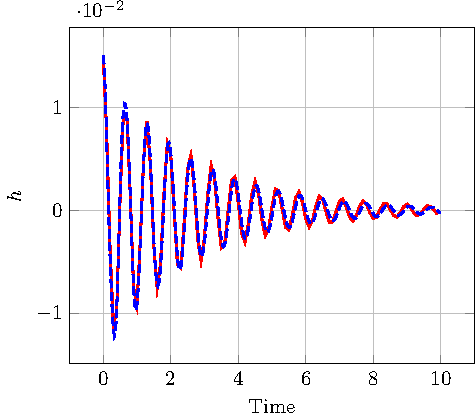
\includegraphics[width=\textwidth]{figures/fig_h_comparison_U_12.pdf}
    \caption{Plunge motion $h$ for $U=12 m/s$.}
  \end{subfigure}
  \begin{subfigure}[]{0.48\textwidth}
    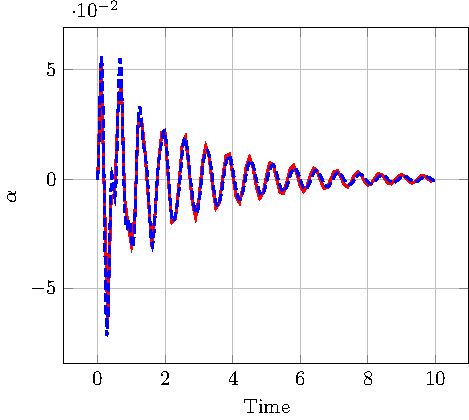
\includegraphics[width=\textwidth]{figures/fig_alpha_comparison_U_12.pdf}
  \caption{Pitch motion $\alpha$ for $U=12 m/s$.}
  \end{subfigure}
  \begin{subfigure}[]{0.48\textwidth}
    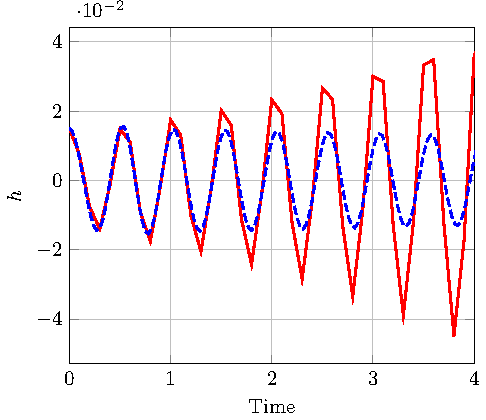
\includegraphics[width=\textwidth]{figures/fig_h_comparison_U_15_3.pdf}
    \caption{Plunge motion $h$ for $U=15.3 m/s$.}
  \end{subfigure}
  \begin{subfigure}[]{0.48\textwidth}
    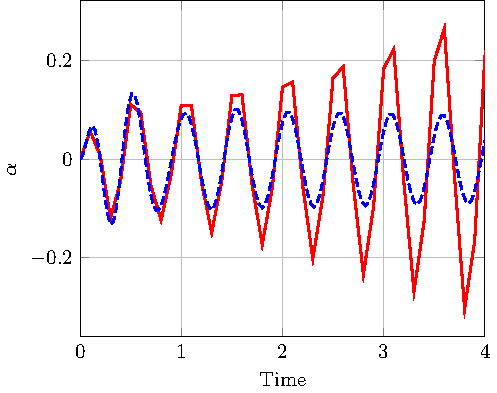
\includegraphics[width=\textwidth]{figures/fig_alpha_comparison_15_3.pdf}
  \caption{Pitch motion $\alpha$ for $U=15.3 m/s$.}
  \end{subfigure}
  \caption{Comparison of the plunge and pitch motions obtained with the LDVM method (red line) and the Theodorsen's model (blue line).}
  \label{fig:validation_dynamical_model}
\end{figure}











\newpage



\bibliographystyle{apalike}
\bibliography{biblio}




\end{document}